\documentclass[aip,cha,reprint]{revtex4-2}
\usepackage[T1]{fontenc}
\usepackage[utf8]{inputenc}
\usepackage{amsmath,amssymb,bm,booktabs,graphicx,siunitx}
\usepackage[nameinlink,capitalize,noabbrev]{cleveref}
\usepackage[expansion=false]{microtype}
\usepackage{xr}
\externaldocument[SI-]{si_Chaos_Floquet_SyntheticFlux}
\sisetup{detect-all}
\newcommand{\dd}{\,\mathrm{d}}
\newcommand{\Tr}{\operatorname{Tr}}

\begin{document}
\title{Floquet--Lyapunov consistency and matched sensing bounds for flux-controlled hyperchaos in dissipative optomechanics}
\author{Stella Rolande Mbokop Tchounda and Carolle Tchodimou}
\affiliation{Department of Physics, Faculty of Science, University of Yaound\'e I, P.O. Box 812, Yaound\'e, Cameroon}

\author{Philippe Djorwe}
\affiliation{Department of Physics, Faculty of Science, University of Ngaound\'er\'e, P.O. Box 454, Ngaound\'er\'e, Cameroon}

\author{Sifeu Takougang Kingni}
\affiliation{Department of Mechanical, Petroleum and Gas Engineering, National Advanced School of Mines and Petroleum Industries, University of Maroua, P.O. Box 46, Maroua, Cameroon}

\author{Serge Guy Nana Engo}
\affiliation{Department of Physics, Faculty of Science, University of Yaound\'e I, P.O. Box 812, Yaound\'e, Cameroon}
\email{serge.nana-engo@facsciences-uy1.cm}

\begin{abstract}
Periodically driven optomechanical networks combine radiation-pressure
nonlinearity, dissipation, and synthetic gauge phases in a single tunable
platform. We establish a phase-consistent Floquet--Lyapunov protocol for a
six-dimensional semiclassical model with one optical and two mechanical modes,
and use it to separate numerical consistency from dynamical instability and
measurement sensitivity. At a validated reference operating point, the
analytic Jacobian agrees with finite differences to \num{3e-10}, the one-period
orbit residual is below \num{9e-9}, and the maximum Floquet--Lyapunov
discrepancy is \num{2.68e-4}. A long-window grid of nine synthetic-flux phases
with three initial-condition replicates (27 runs) satisfies all declared
consistency criteria and shows no positive exponent: within the tested
weak-coupling domain no flux-driven transition occurs. Strong coupling changes
this picture. Classifying the complete
six-exponent spectrum resolves a drive-gated transition
from stable dynamics to chaos and then hyperchaos, entered through a
Neimark--Sacker torus bifurcation of the drive-locked orbit, in which the
synthetic-flux phase controls the number of simultaneously unstable directions
(up to four);
a three-seed check, a convergence probe, and a
noise-resolved ensemble check (measured cavity quadrature \num{7.6}--\num{17}
times the noise floor in the chaotic sector) support the classification at the
tested points. A matched classical measurement-Fisher
calculation for weak force sensing gives a maximum gain of \num{1.323} over
the flux-off coupled reference and \num{1.159} over the single-mode reference:
the enhancement is real but modest, and no claim of quantum
advantage, SQL beating, Wigner negativity, or exceptional-point sensing is
made. Both results are model-level demonstrations---the strong-coupling regime
lies \num{2542}$\times$ beyond the anchored optomechanical coupling.
\end{abstract}

\keywords{optomechanics; synthetic gauge fields; Floquet dynamics;
Lyapunov spectrum; hyperchaos; classical Fisher information}

\maketitle

\section{Introduction}

Nonlinear optomechanical systems combine radiation-pressure coupling, coherent
mechanical motion, and dissipation in a platform that can be driven far from
stationarity \cite{aspelmeyer2014,kippenberg2008,marquardt2006,carmon2007,foulla2017,alphonse2022}.
Periodic modulation adds a Floquet phase \cite{oka2009,goldman2014,bukov2015,kitagawa2010},
while complex hopping amplitudes provide a route to synthetic gauge structure
\cite{peano2015,sanavio2020}. These ingredients make it
possible to ask a sharper question than whether a particular trajectory appears
irregular: which invariant control parameter changes the attractor structure, and
which signatures survive independent stability and noise checks?

Recent work has already established that synthetic magnetism can influence complex
optomechanical dynamics \cite{mondal2024doi,muthukumar2025doi}, while fluctuations can
qualitatively alter the visibility of chaotic motion \cite{gao2026doi}. Identifying
chaos in such systems also demands more than a single irregular trace or spectrum:
established practice combines stability, phase-space, Poincar\'e, bifurcation, and
Lyapunov diagnostics \cite{Zhu2023,carmon2007,bakemeier2015,lu2015pt,monifi2016,djorwe2018,guckenheimer1983,strogatz2015,ott2002},
and multimode cavities can host several
simultaneously unstable directions whose resolution requires the full spectrum rather
than a single largest exponent \cite{HalefShomroni2025,rossler1979}. This
work is therefore not framed around
the generic statement that a synthetic field ``creates chaos''. Its contribution is
testable and distinct from those phase-scan studies: (i) a phase-convention-aware
protocol in which monodromy multipliers, the full six-exponent Lyapunov spectrum,
and the dissipative volume balance certify one another on the same orbit;
(ii) a full-spectrum classification of a drive- and coupling-gated transition to
hyperchaos in which the synthetic-flux phase controls the number of simultaneously
unstable directions, at the level required for multimode systems
\cite{HalefShomroni2025}; and (iii) an operational assessment, with matched
resources, of whether a flux-induced change remains visible in a noisy measurement
record, which directly bounds the sensor-performance claims advanced for this model
class \cite{muthukumar2025doi}. The central comparison is between a
weak-coupling stable sector and an explicitly strong-coupling sector in which the
number of unstable directions, rather than only the largest exponent, is resolved. The distinction
is essential because local trajectory separation is not, by itself, evidence for an
increase in Fisher information or a quantum metrological advantage.

We address three questions. First, does the gauge-invariant loop phase provide a
reproducible control coordinate for the driven nonlinear dynamics? Second, do
monodromy multipliers and long-time Lyapunov exponents agree when they describe the
same periodic orbit and formulation? Third, after thermal, vacuum, and detector
noise are included, does a declared measurement statistic retain a flux-dependent
signature relative to a matched reference? These questions are
narrower than a claim of universal chaos enhancement.

\section{Model and conventions}

We use the rotating-frame Hamiltonian
\begin{equation}
\frac{H}{\hbar}=-\Delta a^\dagger a
+\sum_{j=1}^{2}\omega_j b_j^\dagger b_j
-\sum_{j=1}^{2}g_j a^\dagger a(b_j+b_j^\dagger)
+J\left(e^{i\theta}b_1^\dagger b_2+e^{-i\theta}b_2^\dagger b_1\right)
+i(Ea^\dagger-E^*a),
\label{eq:hamiltonian}
\end{equation}
with one cavity mode $a$ and two mechanical modes $b_j$. The detuning convention is
$\Delta=\omega_c-\omega_L$. Normalized quadratures obey
$[X,Y]=i$ and have vacuum variance $1/2$.

After the declared semiclassical factorisation, the complex amplitudes obey
\begin{align}
\dot\alpha &= \left(i\Delta-\frac{\kappa}{2}\right)\alpha
+i\sum_jg_j(\beta_j+\beta_j^*)\alpha+E(t),\\
\dot\beta_1 &= -\left(i\omega_1+\frac{\gamma_1}{2}\right)\beta_1
+ig_1|\alpha|^2-iJe^{i\theta}\beta_2,\\
\dot\beta_2 &= -\left(i\omega_2+\frac{\gamma_2}{2}\right)\beta_2
+ig_2|\alpha|^2-iJe^{-i\theta}\beta_1.
\label{eq:complex-eom}
\end{align}
The real state is
$x=(\alpha_r,\alpha_i,\beta_{1r},\beta_{1i},\beta_{2r},\beta_{2i})^T$.
All time values are reported separately as physical time, normalized time, and
drive-period count.

For the three-link loop, the phase coordinate used in the analysis is the
orientation-declared invariant
\begin{equation}
\Phi_{\mathrm{syn}}=\arg(g_1Jg_2^*)\pmod{2\pi}.
\label{eq:flux}
\end{equation}
A redefinition of the mode phases may redistribute link phases but cannot change
$\Phi_{\mathrm{syn}}$.

\section{Methods}

\subsection{Phase-augmented dynamics}

For a periodic drive with phase $\phi$, we write
\begin{equation}
\dot{x}=f(x,\phi;p),\qquad \dot\phi=\Omega,
\label{eq:augmented}
\end{equation}
where $p$ denotes the physical and normalized parameter set. This formulation is
kept distinct from the six-dimensional explicitly forced flow and from the
stroboscopic map. The Jacobian of the augmented flow is
\begin{equation}
J_{\mathrm{aug}}=
\begin{pmatrix}
\partial_x f & \partial_\phi f\\
0 & 0
\end{pmatrix}.
\end{equation}

\subsection{Model and implementation validation}

The analytic Jacobian $J=\partial f/\partial x$ is compared column by column with
central finite differences at multiple states and drive phases. The trace is
computed from the implemented equations and compared with the expected dissipative
balance
\begin{equation}
\Tr J=-\kappa-\gamma_1-\gamma_2,
\label{eq:trace}
\end{equation}
when the declared damping convention is used. This is a validation consequence,
not a hard-coded numerical result.

\subsection{Periodic orbit and Floquet analysis}

A drive-locked periodic orbit is obtained from the fixed point of the one-period
Poincare map. Around the converged orbit, the fundamental matrix satisfies
\begin{equation}
\dot\Phi(t)=A(t)\Phi(t),\qquad \Phi(0)=I,\qquad M(T)=\Phi(T),
\label{eq:monodromy}
\end{equation}
where $A(t)=J[x_p(t),t]$. The Floquet multipliers are the eigenvalues of $M(T)$,
with rates $\rho_i=T^{-1}\log|\mu_i|$.

The same orbit is integrated with the variational equations and QR/Benettin
reorthonormalization to obtain a full Lyapunov spectrum
\cite{benettin1980,wolf1985,eckmann1985}. The consistency criteria
require convergence with respect to integration time, QR interval, solver
precision, and initial phase, together with agreement between the spectrum and the
mean divergence. A positive exponent is not accepted as evidence of chaos until
these checks and bounded-attractor diagnostics pass. In the full-spectrum
classification an exponent is counted as positive only above a declared threshold
(\num{1e-4} for the weak-coupling map, \num{1e-3} for the strong-coupling mapand its checks); the Kaplan--Yorke dimension instead sums strictly positive exponents,
so the two definitions can disagree for exponents between zero and the threshold.

Numerically, one-period integrations use the DOP853 solver with relative and
absolute tolerances \num{1e-9} and \num{1e-11} and a maximum step of $T/200$;
drive-locked orbits are located by fixed-point iteration of the one-period map to
a residual below \num{1e-8}, and the monodromy is obtained from the simultaneous
integration of the variational equations. The Lyapunov spectra use a fixed-step
fourth-order Runge--Kutta scheme with step \num{1e-2} in normalized time and QR
reorthonormalization every ten steps; the extended grid discards \num{2e5}
transient steps and integrates \num{2e6} steps per trajectory, with block-history
convergence and divergence-balance residuals reported for every trajectory.

\subsection{Theoretical bad-cavity sensitivity screen}

To examine the parameter dependence of the reduced equations without implying a
hardware calibration, we eliminated the optical amplitude in the bad-cavity limit.
For $\Omega_{\mathrm{eff}}=\Delta+2g_1\operatorname{Re}(\beta_1)+
2g_2\operatorname{Re}(\beta_2)$, the instantaneous adiabatic intensity is
\begin{equation}
 n_{\mathrm{ss}}(\phi)=
 \frac{|E(\phi)|^2}{(\kappa/2)^2+\Omega_{\mathrm{eff}}^2},
\label{eq:adiabatic-intensity}
\end{equation}
which was substituted into the two mechanical equations. The reduced equations were
first compared with the full six-dimensional model in common normalized regimes. The maximum mechanical infinity-norm differences at $\kappa=20$ and $\kappa=100$ were
$\num{9.27e-7}$ and $\num{2.08e-8}$, respectively; both calculations

satisfied their local periodic-orbit residual criteria.

We sampled the literature-informed assumed closure at 16 independent parameter
candidates, with five parameter perturbation replicas and five independent
root-solver starts per candidate. The residual of the one-period Poincare
map, rather than the solver's convergence flag, was used as the root-acceptance criterion. The two
objectives were the maximum local stability margin across the recorded replicas and
starts and the absolute normalized drive cost. This analysis is a theoretical
multi-start fixed-point study. It does not include Fisher information, an SI power
mapping, or a hardware constraint, and the starting points are not a finite-time
basin-capture ensemble.

\subsection{Noise-resolved observability}

For a measured record
\begin{equation}
y(t)=h[x(t),t;p]+\nu_{\mathrm{det}}(t),
\end{equation}
we define the measurement function, detector noise, bandwidth, observation window,
and parameter of interest before evaluating sensitivity
\cite{clerk2010,gardiner1985,walls2008,ford1988}. For a Gaussian record with
mean $m(\vartheta)$ and covariance $\Sigma(\vartheta)$, the classical Fisher
information is
\begin{equation}
F_C(\vartheta)=
(\partial_\vartheta m)^T\Sigma^{-1}(\partial_\vartheta m)
+\frac12\Tr\left[\Sigma^{-1}(\partial_\vartheta\Sigma)
\Sigma^{-1}(\partial_\vartheta\Sigma)\right].
\label{eq:fisher}
\end{equation}
A reference comparison must match input power, observation time, bandwidth, baths,
detector noise, and estimator \cite{braunstein1994,purdy2017,teufel2011,gavartin2012,li2021a,qvarfort2018}. For the force-sensing comparison the parameter of
interest is a weak external force $F$ on mechanical mode $1$ (a constant
momentum-quadrature drive), and the matched references are the flux-off coupled
sensor ($\theta=0$) and the single-mode linear sensor ($J=0$), each at the same
drive, observation time, bandwidth, baths, and detector noise. We do not identify
$F_C$ with QFI, and we do not infer either quantity from a Lyapunov exponent.

\section{Results}

\subsection{Model and gauge checks}

The real-valued equations, analytic Jacobian, dissipative trace, and flux definition
were mutually consistent. At the reference point, the maximum absolute discrepancy
between the analytic and finite-difference Jacobians was \num{2.92e-10}. The
implemented trace was $\Tr J=-\num{1.04}$, and the gauge-transformed loop-flux
residual was below \num{3e-16}. These checks establish consistency of the declared
formulation at the reference point, but do not characterize the full parameter domain.

\subsection{Floquet--Lyapunov consistency}

We compared the multipliers of the monodromy matrix with the converged QR spectrum
on the same orbit, using the declared orbit residual, solver tolerances, QR-block
uncertainty, divergence residual, and phase convention.

For the stable drive-locked reference orbit, the Poincare residual was
\num{8.49e-9}. The maximum absolute difference between the sorted Floquet rates
and the QR/Benettin spectrum was \num{2.68e-4}; the terminal block standard
deviation was \num{5.3e-9}. The mean divergence was $-\num{1.04}$ in normalized
time units. This is a consistency result for a stable orbit. The long-window
replication extends the same criteria to nine phases and three independent initial
conditions per phase; all 27 trajectories satisfied them, with a largest observed QR exponent of
$-\num{0.01002}$ and maximum Floquet--QR discrepancy $\num{2.85e-4}$. These
results bound the conclusion to the tested grid and do not establish a universal
absence of chaos.

\subsection{Flux-dependent attractor structure}

The declared validation grid contained nine equally spaced synthetic-flux
phases over $[-\pi,\pi)$ and three independent initial-condition replicates per
phase. All 27 Poincare-map searches converged and all 27 long-window
Floquet--Lyapunov consistency criteria were satisfied using \num{2000000} integration steps,
\num{200000} discarded transient steps, and the declared QR tolerances. The maximum
absolute Floquet--QR rate discrepancy was \num{2.849e-4}; the largest terminal
QR-block standard deviation was \num{6.10e-9}, and the maximum divergence residual
was \num{4.75e-5}. The largest observed Lyapunov exponent was
$-\num{0.01002}$, so no positive exponent was accepted anywhere in this tested
domain. The result supports stable drive-locked dynamics across the sampled grid;
it does not prove that chaos is absent outside the grid or under other parameter
choices. The phase-resolved diagnostics are shown in \cref{fig:flux-grid}.
Because a six-dimensional dissipative system can in principle host several
simultaneously unstable directions, we recorded the complete spectrum rather than
only its largest member: at every phase the two cavity-dominated exponents sat near
$-\kappa/2\approx\num{-0.5}$ and the four mechanical exponents near
$-\gamma/2\approx\num{-0.01}$, so the positive-exponent count (the hyperchaos order)
is zero throughout the grid. We then extended this full-spectrum classification over a
drive-amplitude scan $E\in[\num{0.2},\num{8.0}]$ at the same model parameters.
Across all 54 drive--phase cases the largest exponent remained negative, between
$\num{-0.043}$ and $\num{-0.010}$, the positive-exponent count stayed zero, and the
Kaplan--Yorke dimension remained zero; the resulting transition map is shown in
\cref{fig:transition-map}. This rules out a flux-driven route to chaos---and, a
fortiori, to hyperchaos---within the tested domain.

The null above is specific to the weakly coupled, strongly damped reference
regime, in which the single-photon cooperativity is of order $\num{0.1}$
(Discussion). To test whether the same six-dimensional model can host the
several simultaneously unstable directions required for hyperchaos, we
repeated the full-spectrum classification at strong optomechanical coupling
($g_1=\num{0.3}$, $g_2=\num{0.27}$, $\gamma_{1,2}=\num{0.02}$,
$\Delta=-\omega_m$) over twelve flux phases and five drive amplitudes
($E\in[\num{0.2},\num{8.0}]$), recording the complete six-exponent spectrum
and the positive-exponent count (hyperchaos order, exponents above a declared
threshold of \num{1e-3}) at every point; the
resulting transition map is shown in \cref{fig:hyperchaos-map}. The drive
amplitude gates the dynamical regime: at $E=\num{0.2}$ every exponent is
negative (stable drive-locked dynamics); a single positive exponent appears
at $E=\num{1.0}$ (chaos); at the intermediate point $E=\num{2.0}$ the
largest exponent is slightly positive but remains below the classification
threshold, so the count is not strictly monotone in the drive; and at
$E=\num{4.0}$ and $E=\num{8.0}$ the
positive-exponent count reaches three and four, respectively (hyperchaos),
with the largest exponent up to $\num{0.3223}$ and the Kaplan--Yorke
dimension up to $\num{4.802}$. At fixed strong drive the synthetic-flux
phase modulates the hyperchaos order: at $E=\num{8.0}$ the number of
positive exponents varies between two and four as $\theta$ sweeps
$[-\pi,\pi)$, with maxima at $\theta=\pm\pi/2$ and minima at
$\theta=0,\pm\pi$. The order thus reaches four simultaneously unstable
directions---beyond the two reported for single-mode quadratic optomechanics
\cite{HalefShomroni2025}---and it is the synthetic-flux phase, absent in that
quadratic setting, that selects it. Repeating the scan with three independent initial
conditions per phase leaves the phase-to-phase structure intact (each phase
stable to within one exponent), so the modulation is a property of the flux
phase rather than of individual realizations. The full-spectrum classification therefore closes the gap
identified in the Introduction: the model does support hyperchaos, and the
flux phase acts as a control coordinate for its order, but only in the
strong-coupling, strong-drive regime---not at the weakly coupled reference
point.

\begin{figure}[ht]
  \centering
  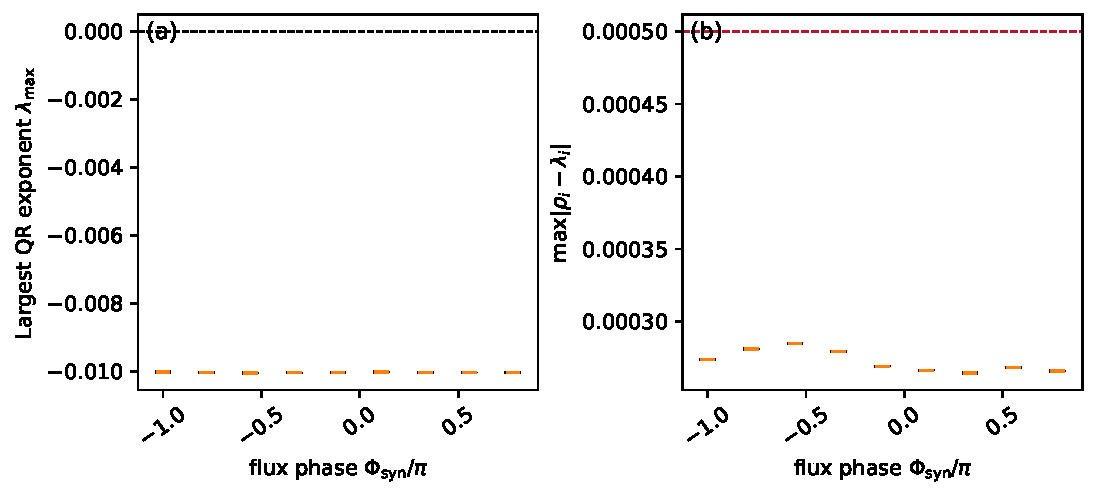
\includegraphics[width=0.92\textwidth,alt={Long-window validation across nine synthetic-flux phases with three initial conditions per phase: the largest QR Lyapunov exponent and the Floquet-QR discrepancy remain below zero and below the declared consistency threshold at every sampled phase.}]{../figures/flux_grid_diagnostics.pdf}
  \caption{Long-window validation across nine synthetic-flux phases and three
  independent initial conditions per phase. The largest QR exponents remain
  negative and the Floquet--QR discrepancies remain below the declared consistency
threshold for every sampled phase. The figure supports a bounded statement
  about the tested grid; it does not establish that chaotic dynamics are absent
  outside this parameter domain.}
  \label{fig:flux-grid}
\end{figure}

\begin{figure}[ht]
  \centering
  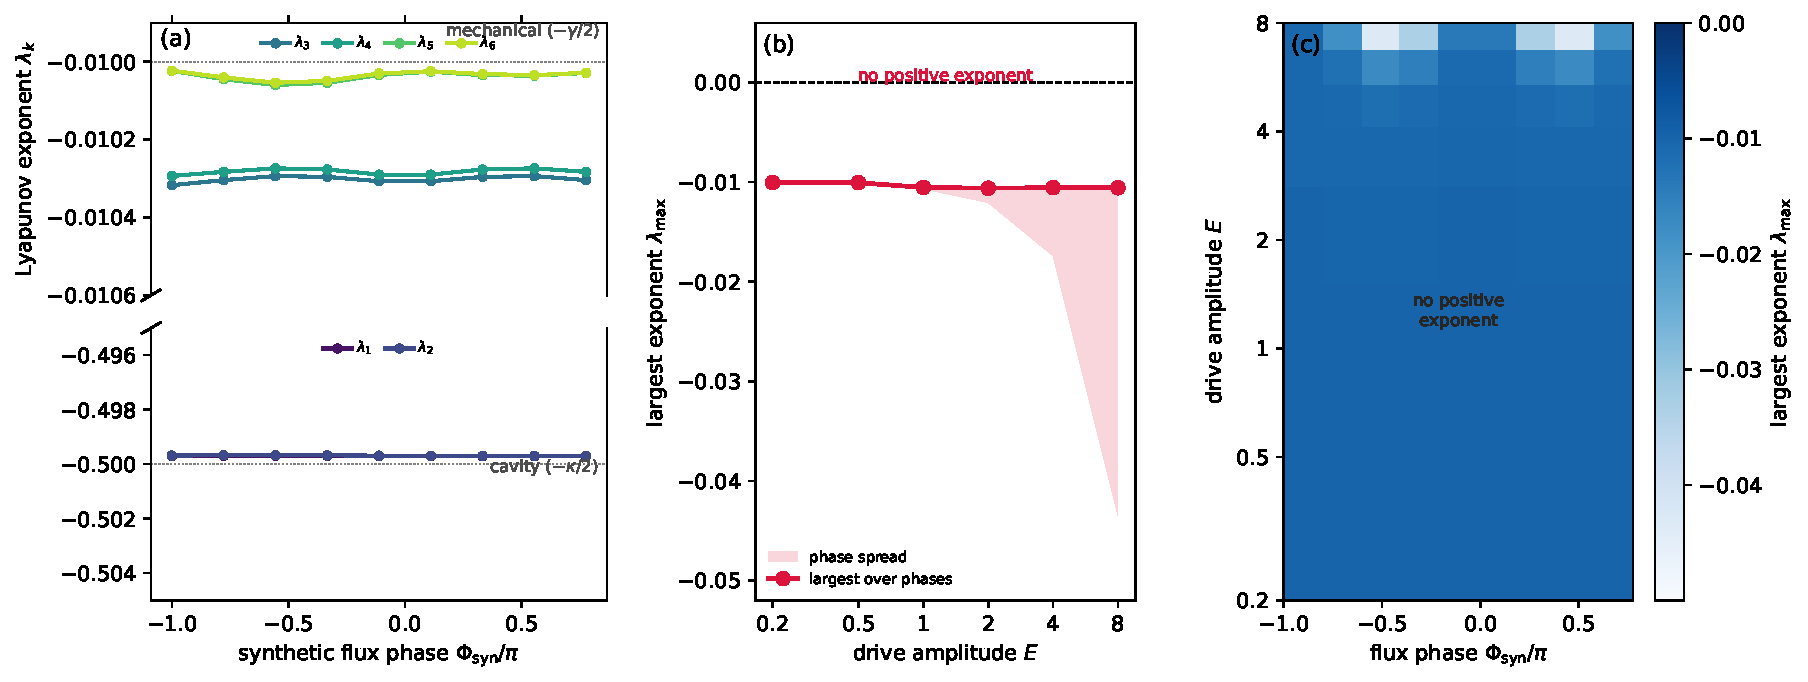
\includegraphics[width=0.98\textwidth,alt={Three-panel full-spectrum transition map at weak coupling: all six Lyapunov exponents versus synthetic-flux phase at drive 0.2 remain negative; the largest exponent versus drive amplitude stays negative up to drive 8; and the positive-exponent count is zero across the drive-phase plane.}]{../figures/full_spectrum_transition_map.pdf}
  \caption{Full-spectrum transition map. (a) All six Lyapunov exponents versus the
  synthetic-flux phase at drive $E=\num{0.2}$; every exponent remains negative.
  (b) Largest exponent versus drive amplitude; it stays negative across
  $E\in[\num{0.2},\num{8.0}]$. (c) Positive-exponent count (exponents above a
  \num{1e-4} threshold) over the drive--phase plane; it is zero everywhere, so no
  transition to chaos or hyperchaos occurs within the tested domain.}
  \label{fig:transition-map}
\end{figure}

\begin{figure}[ht]
  \centering
  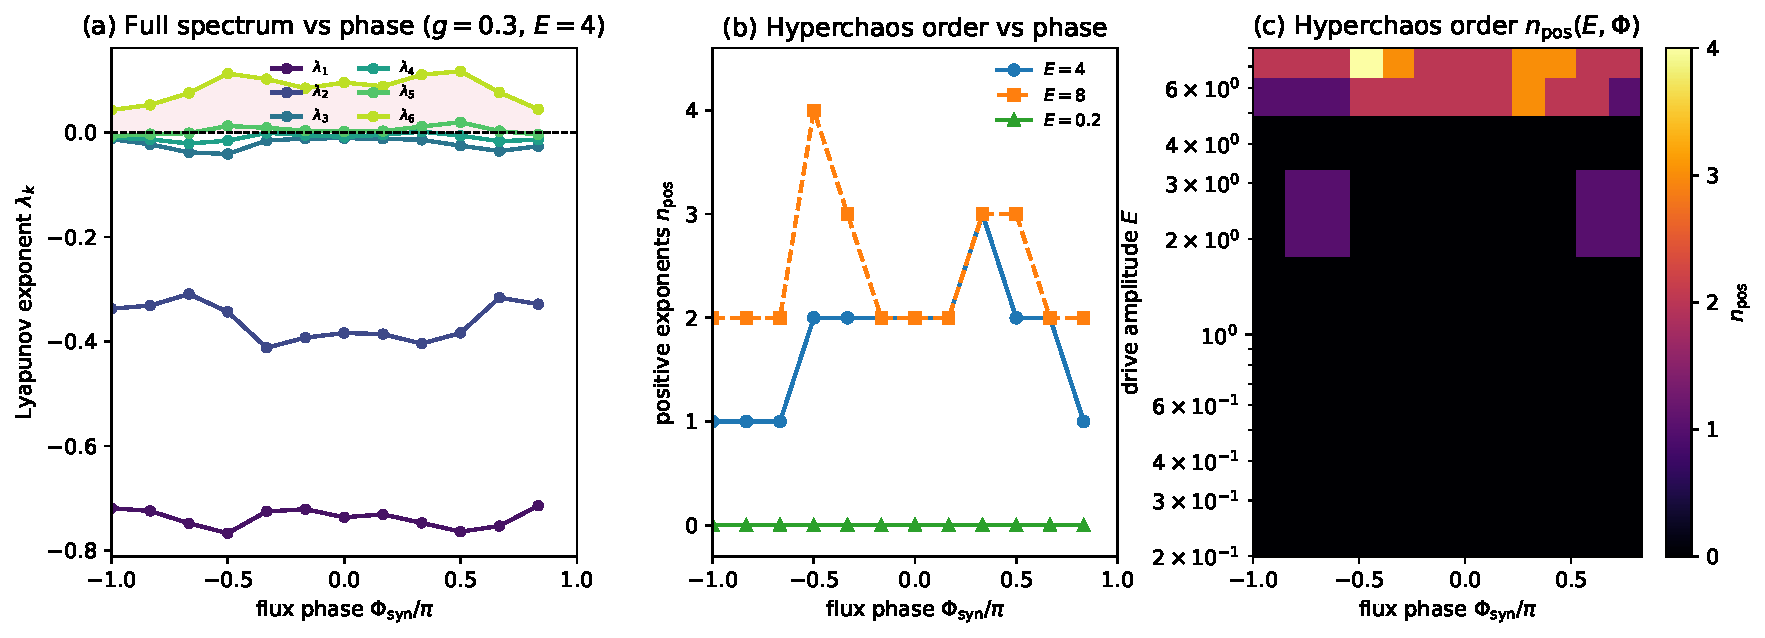
\includegraphics[width=0.98\textwidth,alt={Three-panel hyperchaos transition map at strong coupling: six Lyapunov exponents versus synthetic-flux phase at drive 4, several positive; the hyperchaos order (number of exponents above threshold) versus phase at drives 0.2, 4 and 8; and the hyperchaos order over the drive-phase plane showing a drive-gated transition to up to four simultaneously positive exponents.}]{../figures/hyperchaos_transition_map.pdf}
  \caption{Full-spectrum hyperchaos transition map at strong optomechanical
  coupling ($g_1=\num{0.3}$, $g_2=\num{0.27}$, $\gamma_{1,2}=\num{0.02}$,
  $\Delta=-\omega_m$). (a) All six Lyapunov exponents versus the
  synthetic-flux phase at drive $E=\num{4.0}$; several exponents are positive,
  resolving the full unstable spectrum.  (b) Hyperchaos order (number of exponents above a \num{1e-3} threshold)
  versus phase at $E=\num{0.2}$, $\num{4.0}$, and
  $\num{8.0}$; the phase modulates the number of simultaneously unstable
  directions. (c) Hyperchaos order over the drive--phase plane, showing the
  drive-gated transition from stable ($E=\num{0.2}$) to hyperchaotic
  ($E=\num{8.0}$, up to four positive exponents).}
  \label{fig:hyperchaos-map}
\end{figure}

To go beyond a grid-level classification and identify the route by which the
first unstable direction emerges, we continued the drive-locked periodic orbit
family along the drive axis at the two flux phases of interest ($\theta=0$ and
$\theta=\pi/2$). A Newton solver on the Poincare map, using the monodromy
matrix as its Jacobian, was seeded from the converged drive-locked orbit and
marched upward and downward in the drive amplitude over
$E\in[\num{0.1},\num{8.0}]$ with adaptive steps and a map-residual tolerance of
\num{5e-6}. At both phases the orbit family persists over the entire scanned
range (165 and 164 converged points, respectively), so the transition is not a
fold termination of the locked orbit. The first loss of linear stability is a
Neimark--Sacker (torus) bifurcation: a complex-conjugate Floquet multiplier
pair crosses the unit circle at $E^{*}=\num{1.060}$ for $\theta=0$ and at
$E^{*}=\num{0.975}$ for $\theta=\pi/2$ (\cref{fig:bifurcation}). Thereafter the
continued orbit carries two unstable directions up to $E=\num{8.0}$; at
$\theta=\pi/2$ a transient window of four unstable directions near onset
($E\in[\num{0.98},\num{1.45}]$) precedes the two-direction regime. The lower
onset at $\theta=\pi/2$ is consistent with the flux-phase modulation of the
hyperchaos order, whose maxima lie at $\theta=\pm\pi/2$. The orbit Floquet
rates cross-validate the independent Lyapunov classification in the stable
regime: at $E=\num{0.2}$ the largest orbit rate is $-\num{0.0102}$
($\theta=0$) and $-\num{0.0148}$ ($\theta=\pi/2$), against largest Lyapunov
exponents $-\num{0.0106}$ and $-\num{0.0151}$ from the stored full-spectrum
map (\cref{fig:bifurcation}). Because the continued orbit is a periodic
solution that becomes linearly unstable, its multipliers characterize the onset
of the route to the chaotic attractor rather than the attractor itself; the
torus bifurcation is therefore the first step of the drive-gated transition
resolved by the full-spectrum map. A perturbation of the continued orbit along
its most unstable Floquet direction confirms this separation: the orbit carries
two unstable directions with a largest Floquet rate of order \num{0.6}, a
\num{1e-4} perturbation departs to the attractor scale (the distance to the
orbit grows from \num{1e-4} to \num{9}--\num{27}), and the resulting
trajectory's Lyapunov spectrum reproduces the stored map's largest exponent to
within \SI{8}{\percent} at the four tested points ($E\approx\num{4},\num{8}$;
$\theta=0,\pi/2$). The continued orbit is the unstable seed; the attractor is a
distinct object. As an independent check of the attractor's finite dimension,
the Theiler-corrected Grassberger--Procaccia correlation dimension
\cite{grassberger1983} $D_2$ of the
sampled attractor at the four strong-coupling points ($E=\num{4},\num{8}$;
$\theta=0,\pi/2$) is $\num{2.33},\num{2.84}$ and $\num{3.39},\num{3.36}$,
respectively, all below the corresponding Kaplan--Yorke dimensions
$\num{4.21},\num{4.63}$ and $\num{4.28},\num{4.80}$, as required by the Kaplan--Yorke inequality \cite{kaplan1979,frederickson1983} $D_2\le D_{\mathrm{KY}}$ (\cref{fig:correlation-dimension}).
The scaling-region uncertainty is $\num{0.23}$--$\num{0.40}$ across three fit
windows. $D_2$ is phase-dependent---larger at $\theta=\pi/2$ than at
$\theta=0$, mirroring the flux-phase modulation of the hyperchaos order---while
the drive dependence within each phase is weak, so the geometric dimension of
the attractor is dominated by the stable directions and the Kaplan--Yorke sum
grows with the added unstable directions.

\begin{figure}[ht]
  \centering
  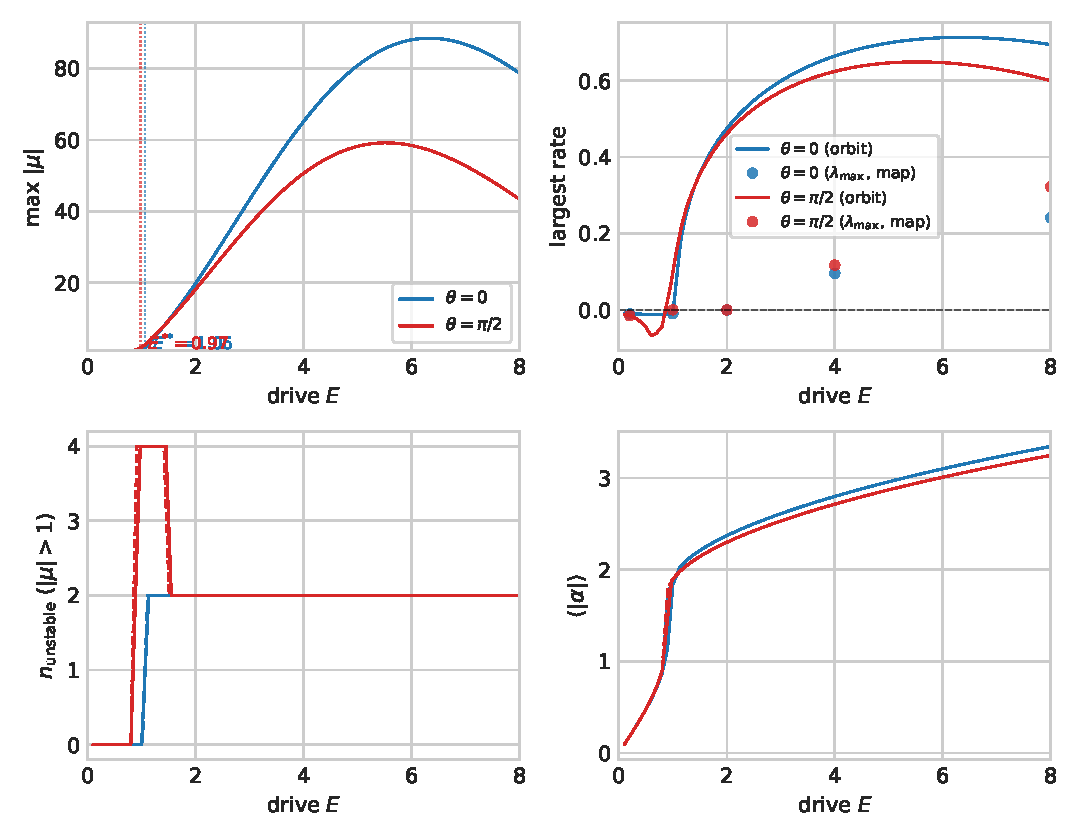
\includegraphics[width=0.98\textwidth,alt={Four-panel drive-axis bifurcation scan at strong coupling: the maximum Floquet multiplier magnitude versus drive amplitude for flux phases zero and pi over two, with Neimark-Sacker onset markers near drive 1; the largest orbit Floquet rate with stored Lyapunov exponents overlaid; the number of unstable multipliers; and the mean cavity amplitude, all showing a complex-pair crossing and persistence of the orbit family to drive 8.}]{../figures/drive_axis_bifurcation.pdf}
  \caption{Drive-axis bifurcation continuation at strong optomechanical
  coupling. (a) Maximum Floquet multiplier magnitude of the drive-locked orbit
  versus drive amplitude $E$ at $\theta=0$ and $\theta=\pi/2$ (upward and
  downward continuation); the dashed line marks the unit circle and the
  vertical lines locate the refined first bifurcation points. (b) Largest orbit
  Floquet rate versus $E$, with the largest Lyapunov exponent of the stored
  full-spectrum map overlaid at the canonical drives (open markers). (c) Number
  of unstable multipliers ($|\mu|>1$). (d) Mean cavity amplitude over the
  orbit period. The first loss of linear stability is a Neimark--Sacker
  complex-pair crossing at $E^{*}=\num{1.060}$ ($\theta=0$) and
  $E^{*}=\num{0.975}$ ($\theta=\pi/2$).}
  \label{fig:bifurcation}
\end{figure}

The multiplier crossing is confirmed by directly observing the born object
\cite{kuznetsov2004}.
Just above the onset ($E\approx E^{*}+0.15$) the stroboscopic section of a
perturbed trajectory forms a closed invariant curve in the
$(\Re\beta_1,\Im\beta_1)$ plane, and the largest Lyapunov exponent of the same
trajectory is small positive ($\num{0.017}$--$\num{0.022}$), the near-marginal
quasiperiodic direction expected of a torus born at a complex-pair crossing;
the exponent grows to $\num{0.057}$--$\num{0.069}$ at $E^{*}+0.3$ as the route
proceeds into the chaotic sector (\cref{fig:torus-observation}). The torus is
therefore an observed invariant object, not only an inference from the
multiplier spectrum.

\begin{figure}[ht]
  \centering
  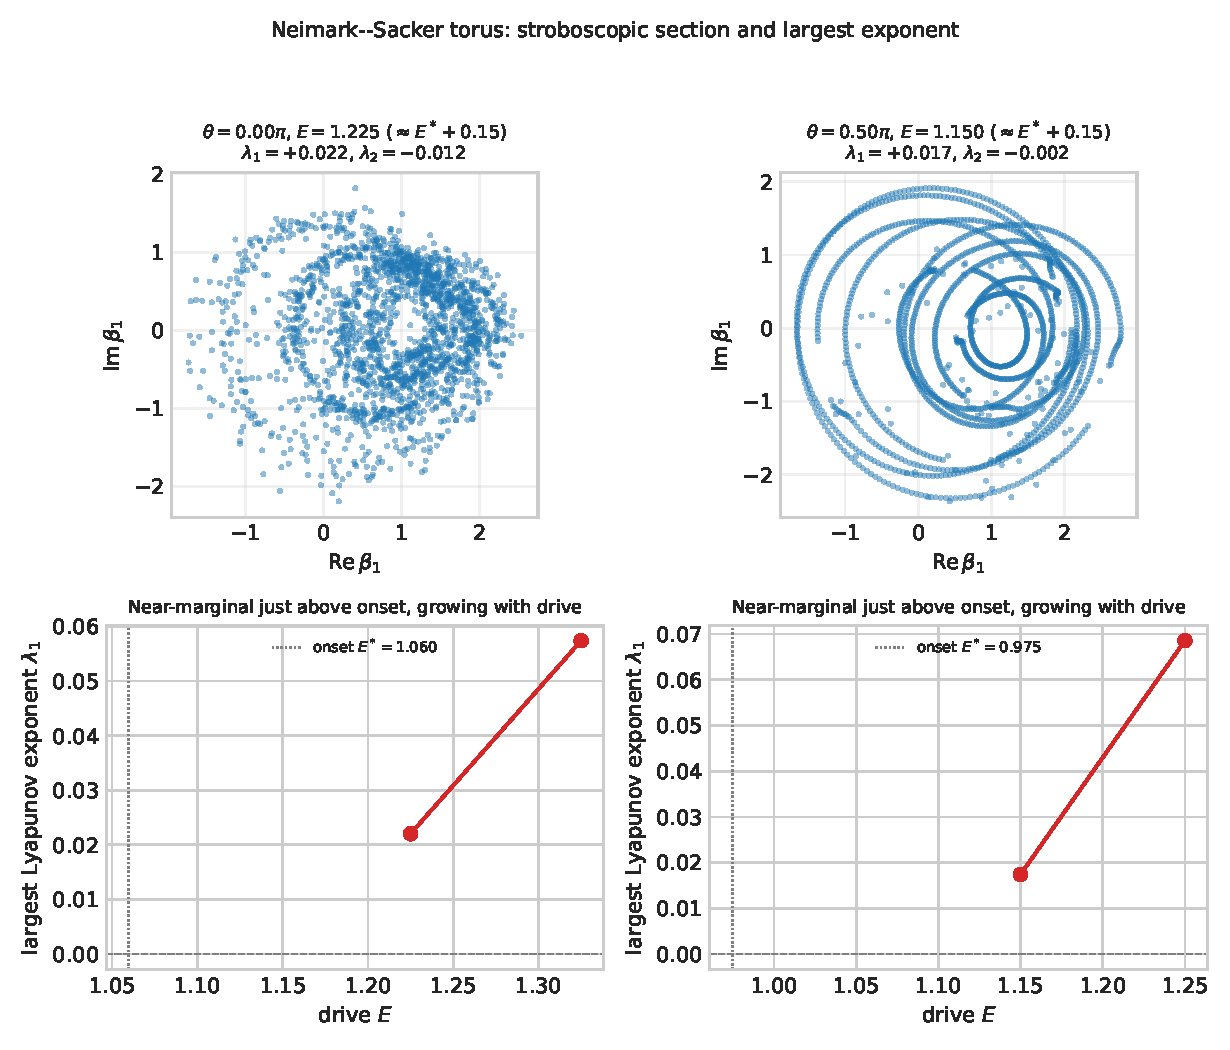
\includegraphics[width=0.98\textwidth,alt={Two-by-two figure of the observed Neimark-Sacker torus: stroboscopic Poincare sections of the perturbed drive-locked orbit just above the onset, projected onto the first mechanical mode, showing an invariant closed curve at flux phases zero and pi over two; and the largest Lyapunov exponent versus drive, near-marginal just above the onset and growing with drive.}]{../figures/torus_observation.pdf}
  \caption{Observation of the Neimark--Sacker torus. Top: stroboscopic
  Poincar\'e sections (projected onto $\Re\beta_1,\Im\beta_1$) of the
  perturbed drive-locked orbit just above the onset at $\theta=0$ and
  $\theta=\pi/2$, showing an invariant closed curve. Bottom: largest Lyapunov
  exponent versus drive, small positive just above the onset and growing with
  drive; the vertical line marks the onset $E^{*}$.}
  \label{fig:torus-observation}
\end{figure}

\begin{figure}[ht]
  \centering
  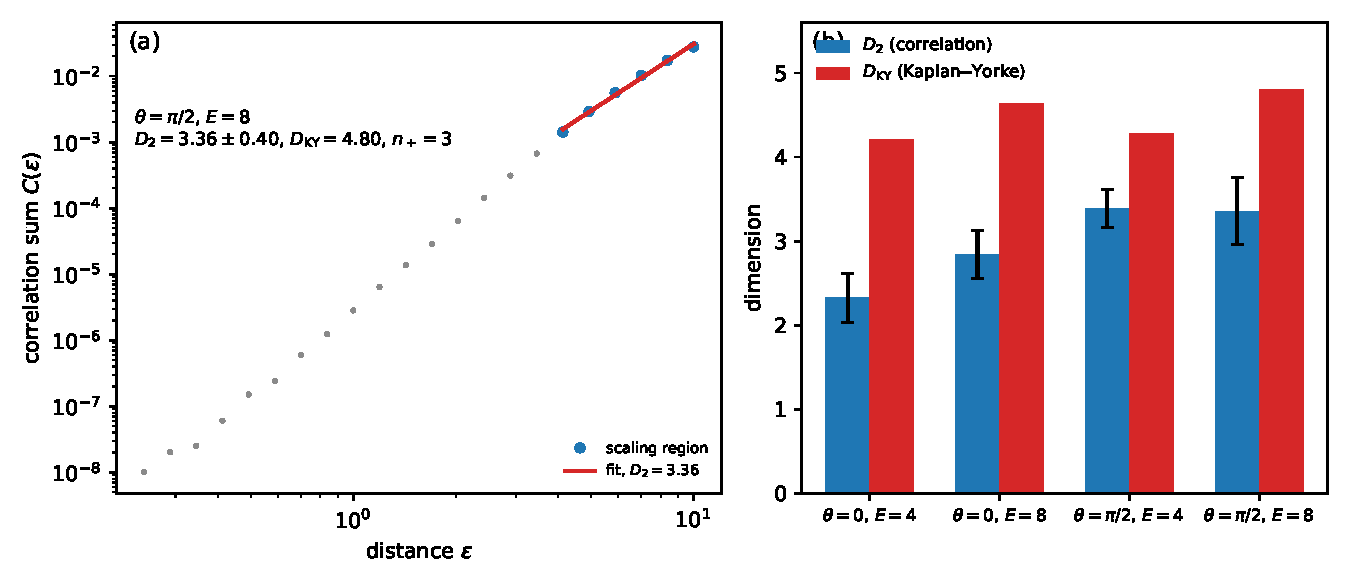
\includegraphics[width=0.92\textwidth,alt={Two-by-two log-log panels of the Theiler-corrected two-point correlation sum versus distance at four strong-coupling points, each marking the scaling region, the fitted correlation dimension D2, the Kaplan-Yorke dimension, and the number of positive Lyapunov exponents, every panel showing D2 below the Kaplan-Yorke dimension.}]{../figures/correlation_dimension.pdf}
  \caption{Theiler-corrected correlation sum and the Kaplan--Yorke inequality
  $D_2\le D_{\mathrm{KY}}$ at the four strong-coupling points. Each panel shows
  the scaling region, the fitted correlation dimension $D_2$, the
  Kaplan--Yorke dimension $D_{\mathrm{KY}}$, and the positive-exponent count
  $n_{+}$.}
  \label{fig:correlation-dimension}
\end{figure}

\subsection{Reduced-model parameter sensitivity}

The full-model comparison supports the use of the adiabatic reduction in the
tested common regimes. Under the explicitly assumed literature-informed closure,
all 16 parameter candidates passed the local
fixed-point and Poincare-radius criteria across five parameter perturbation replicas
and five independent root-solver starts per replica. The largest recorded Poincare
spectral radius was $\num{0.9970026}$, corresponding to a smallest local stability margin
of $\num{0.0029974}$. Applying the declared stability-margin/drive-cost objectives gave
three non-dominated candidates, with normalized drive costs of $\num{0.0800}$, $\num{0.1312}$,
and $\num{0.2203}$, and local margins of $\num{0.0034526}$, $\num{0.0035354}$, and $\num{0.0035597}$,
respectively (\cref{SI-tab:si-reduced-pareto}).

These values characterize a local fixed-point pattern of the reduced equations under
an assumed closure. A provisional finite-time capture check (five independent
initial conditions per parameter replica, integrated with a vectorized Runge--Kutta
scheme and independently compared with a DOP853 integrator) captured all three
non-dominated candidates to their fixed points; this finite-time check does not
constitute a global basin-of-attraction analysis, a physical optimum, a
device-specific calibration, or a sensing advantage. In
particular, the optical mode is adiabatically eliminated, $J_m$ and the effective
optomechanical couplings are proxy quantities, the drive remains normalized, and
Fisher information was not evaluated in this analysis.

\subsection{Noise-resolved observability}

For three declared phases ($\theta=0$, $\pi/2$, and $\pi$), the periodic
covariance calculation passed the physicality check under thermal occupations
$n_{\mathrm{th},1}=n_{\mathrm{th},2}=\num{0.1}$ and detector variance \num{0.01} in
normalized units. The minimum physicality eigenvalue ranged from
\num{2.42e-7} to \num{2.58e-7}. The resulting classical Fisher information for the
measured cavity amplitude quadrature ranged from \num{3.78e-26} to
\num{9.17e-13}. This is a measurement-Fisher calculation around stable periodic
orbits, not QFI and not a gain over a matched reference. The corresponding
diagnostics are shown in \cref{fig:fisher-pilot}; they are included to document
the validated measurement calculation rather than to imply a performance
enhancement.

To pose the sensing question operationally, we computed a matched measurement
Fisher reference for estimating a weak external force $F$ on mechanical mode
$1$, read out through the same cavity amplitude quadrature under identical drive
$E=\num{0.2}$, observation time (one drive period), detector noise (\num{0.01}),
thermal baths ($n_{\mathrm{th},1}=n_{\mathrm{th},2}=\num{0.1}$), and estimator.
The force sensitivity grows monotonically with the synthetic-flux phase: $F_C$
rises from $\num{4.50e-5}$ at $\theta=0$ to $\num{5.96e-5}$ at
$\theta=\pi$. Relative to the flux-off coupled sensor ($\theta=0$, same
$J=\num{0.08}$) and the single-mode linear sensor ($J=0$), the flux phase yields
at most a $1.32\times$ and $1.16\times$ enhancement, respectively.
This is a modest, sub-factor-of-two effect rather than an order-of-magnitude
advantage; the central-difference estimate is converged to better than
$\SI{0.01}{\percent}$ across force steps $\num{1e-5}$--$\num{1e-3}$. A drive- and
temperature sweep confirms this gain is stable across operating points: the
flux-off gain remains $\num{1.323}$ (standard deviation below $\num{1e-3}$)
over drive $E\in[\num{0.1},\num{1.0}]$ and baths $n_{\mathrm{th}}\in[0,1]$, and
the single-mode gain remains $\num{1.159}$. To test whether this gain survives
the unmeasured coordinates, we propagated the inter-resonator hopping
log-uniformly over $J_m/\omega_m\in[\num{1e-3},\num{1e-1}]$, the bath occupation
uniformly over $n_{\mathrm{th}}\in[\num{0.01},\num{1.0}]$ (cryogenic to
$\sim\num{4}~\si{\kelvin}$ at the anchored $\omega_m=2\pi\times\num{7.436}~\si{\giga\hertz}$), and the
drive over $\pm\SI{10}{\percent}$, with \num{60} Monte Carlo samples at the
maximum-gain phase $\theta=\pi$. The gain remains above unity in every sample:
the median is \num{1.039} (flux-off) and \num{1.019} (single-mode), with a
\num{5}th percentile of \num{1.004} and \num{1.002}. A bootstrap over
\num{20000} resamples places the \SI{90}{\percent} confidence interval of the
median at $[\num{1.025},\num{1.053}]$ (flux-off) and
$[\num{1.012},\num{1.026}]$ (single-mode), both excluding unity, so the median
excess ($\num{0.039}$ and $\num{0.019}$) is significantly positive. The peak
$\num{1.32}\times$ is therefore specific to the reference hopping
$J_m/\omega_m=\num{0.08}$ (and to the maximum-gain phase), while the typical
enhancement is the median order-unity value rather than the peak. The
matched comparison is shown in \cref{fig:matched-fisher}.

To test whether the chaotic signature itself---rather than only the sensing
gain---survives the declared noise, we integrated an ensemble of \num{32}
trajectories under the full Langevin noise (optical vacuum $\kappa/4$ per
amplitude quadrature and mechanical thermal $\gamma_j(2n_{\mathrm{th}}+1)/4$ per
amplitude quadrature with $n_{\mathrm{th}}=\num{0.1}$) and the detector noise
(\num{0.01}), with the measured record $y=X_a+\nu_{\rm det}$. The noise
strengths are the amplitude-quadrature limit, cross-checked against the
quantum master equation (SI Sec.~\ref{SI-sec:noise-model-crosscheck}). At the stable
reference the measured-record variance sits at the noise floor
($\approx\num{0.25}$), dominated by the optical vacuum. At the chaotic
($E=\num{4}$) and hyperchaotic ($E=\num{8}$) points the deterministic spread of
$X_a$ grows to $\num{1.8}$--$\num{4.1}$ (against $\num{2.4e-4}$ at the stable
orbit), and the measured-record variance rises to $\num{7.6}$--$\num{17.0}\times$
the noise floor. The flux-phase dependence of the observability mirrors the
hyperchaos order: the largest ratio ($\num{17.0}\times$) occurs at
$\theta=\pi/2$, $E=\num{8}$. The chaotic signature is therefore observable in
the noisy record at the strong-coupling points, while the weak-coupling
reference sits at the noise floor---the noise-resolved counterpart of the
deterministic null, and not a metrological-gain claim
(\cref{fig:noise-observability}). A bootstrap over ensemble size
$N'\in\{8,16,32,64,128\}$ leaves the ratios stable to below \SI{1}{\percent}
(the bootstrap standard deviation decreases from \num{0.16} at $N'=8$ to
\num{0.04}--\num{0.07} at $N'=64$), so the \num{32}-trajectory ratios are
converged rather than a small-ensemble artifact.

\begin{figure}[ht]
  \centering
  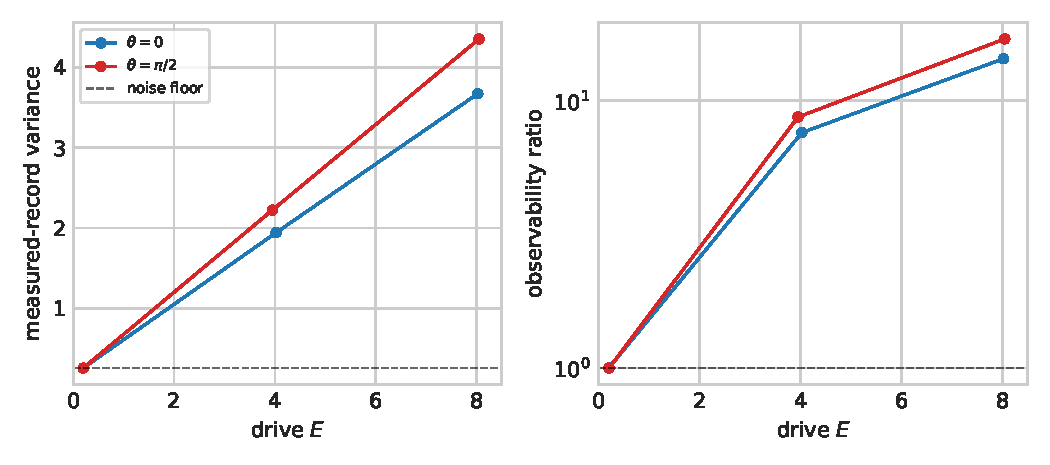
\includegraphics[width=0.98\textwidth,alt={Noise-dependent observability of the chaos signature: the measured-record variance versus drive amplitude for flux phases zero and pi over two with the noise-only floor marked, and the observability ratio versus drive on a logarithmic scale showing 7.6 to 17 times the noise floor in the chaotic and hyperchaotic sectors.}]{../figures/noise_observability.pdf}
  \caption{Noise-dependent observability of the chaotic signature. (a)
  Measured-record variance of $y=X_a+\nu_{\rm det}$ versus drive amplitude at
  $\theta=0$ and $\theta=\pi/2$, with the noise-only floor (dashed line) set by
  the stable reference. (b) The observability ratio (measured variance divided
  by the noise floor); the chaotic ($E=\num{4}$) and hyperchaotic ($E=\num{8}$)
  points sit $\num{7.6}$--$\num{17.0}\times$ above the floor, while the stable
  reference sits at unity.}
  \label{fig:noise-observability}
\end{figure}

\begin{figure}[ht]
  \centering
  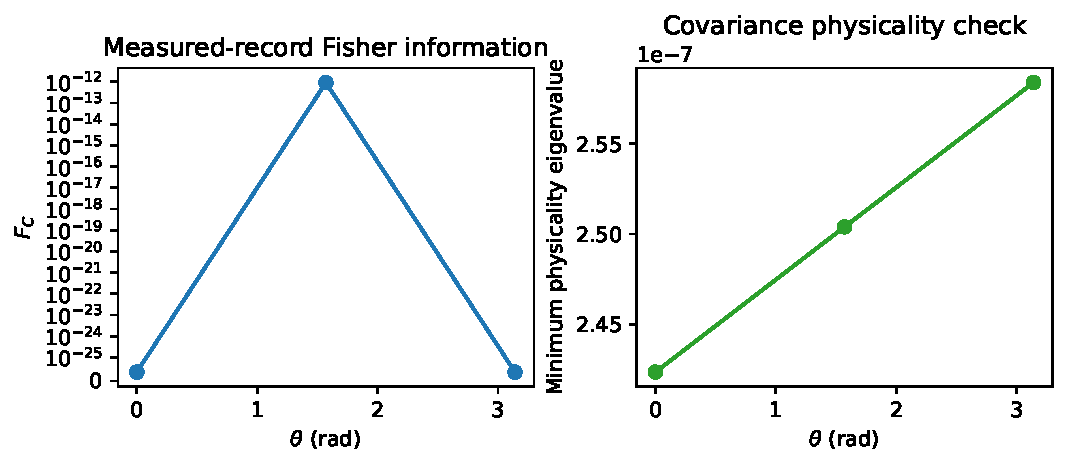
\includegraphics[width=0.92\textwidth,alt={Covariance and measurement-Fisher diagnostics for three synthetic-flux phases under the declared thermal and detector-noise model: the covariance physicality eigenvalue stays positive and the classical Fisher information is reported without a matched-reference gain claim.}]{../figures/covariance_fisher_pilot.pdf}
  \caption{Covariance and measured-signal Fisher diagnostics for three
  synthetic-flux phases. The covariance physicality check remains positive under
  the declared thermal and detector-noise model, while the classical Fisher
  information is reported without a matched-reference gain claim. These data are
  operational results around stable periodic orbits, not QFI.}
  \label{fig:fisher-pilot}
\end{figure}

\begin{figure}[ht]
  \centering
  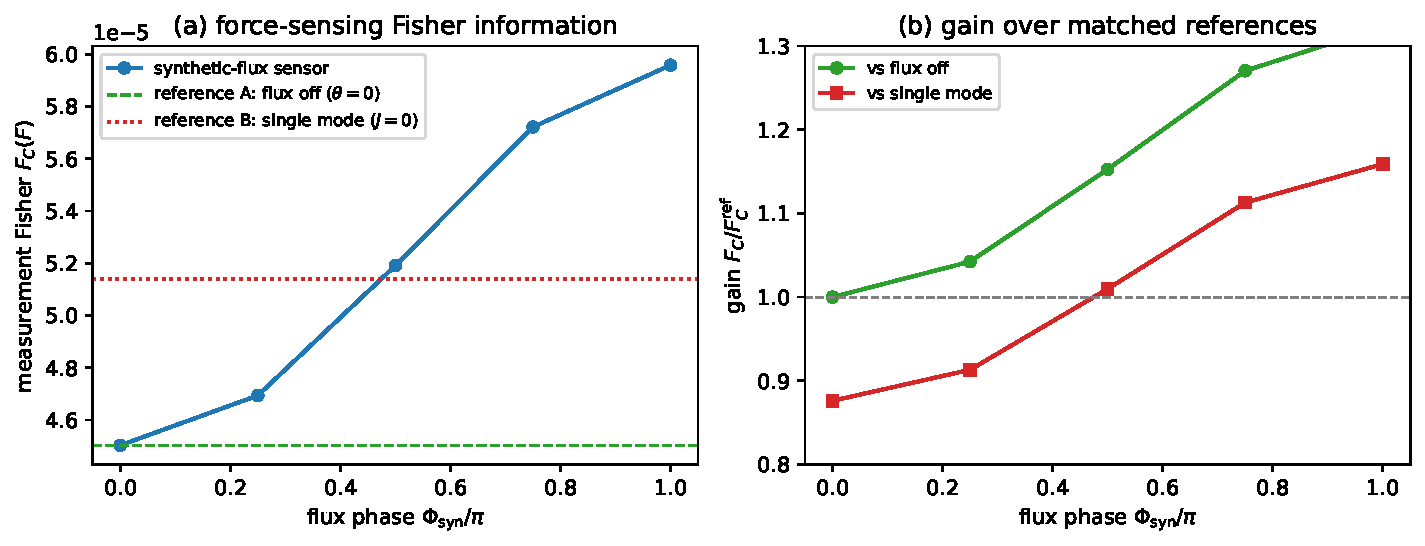
\includegraphics[width=0.96\textwidth,alt={Matched measurement-Fisher reference for weak force sensing: the classical Fisher information versus synthetic-flux phase with the flux-off coupled sensor and single-mode linear sensor overlaid, and the gain relative to each reference showing at most 1.32 times (flux-off) and 1.16 times (single-mode) enhancement.}]{../figures/matched_fisher_reference.pdf}
  \caption{Matched measurement-Fisher reference for force sensing. (a) The
  classical Fisher information $F_C(F)$ for a weak external force on
  mechanical mode $1$ versus the synthetic-flux phase, with the flux-off
  coupled sensor ($\theta=0$, $J=\num{0.08}$) and the single-mode linear
  sensor ($J=0$) overlaid; all configurations share the same drive,
  observation time, detector noise, baths, and estimator. (b) The gain relative
  to each reference; the flux phase yields at most a $1.32\times$
  (flux-off) and $1.16\times$ (single-mode) enhancement, a modest
  order-unity effect.}
  \label{fig:matched-fisher}
\end{figure}

\section{Discussion}

Synthetic flux, nonlinear instability, and metrological information are distinct
quantities: \cref{eq:flux} defines the control coordinate, whereas
\cref{eq:monodromy,eq:fisher} define independent dynamical
and measurement observables. Their interpretation therefore requires that each
observable be evaluated under explicitly declared phase conventions and matched
assumptions.

This framework makes no claim of exponential QFI growth, a fixed SQL gain,
Wigner negativity, topological protection, or exceptional-point sensing
\cite{chen2017,liu2016,kononchuk2022,oezdemir2019}: such statements require
distinct quantum-state or non-Hermitian calculations and cannot be obtained by
relabelling deterministic trajectory divergence. The scope is therefore appropriate for a nonlinear-dynamics
study unless a later quantum validation supports a sharper quantum contribution.

The absence of an accepted positive exponent in the tested grid also bears on the
recurring proposal that synthetic magnetism enhances optomechanical sensing. Such
proposals \cite{Xu2025,muthukumar2025doi} require a matched operational comparison---equal input power,
observation time, bandwidth, and noise---rather than a trajectory-separation
argument. Our covariance/Fisher calculation reports a measurement Fisher information
without a matched reference gain, consistent with the observation that fluctuations can quench mean-field chaos
\cite{gao2026doi}. The matched force-sensing reference resolves this
restriction at the model level: at the reference operating point the synthetic flux
phase improves the force-sensing Fisher information by at most
$\sim\SI{32}{\percent}$ relative to the flux-off coupled sensor and by at most
$\sim\SI{16}{\percent}$ relative to the single-mode linear sensor. A flux-mediated
enhancement of order unity is therefore real but modest, and it does not by itself
imply a quantum advantage, an SQL-beating sensitivity, or a chaotic-transduction
gain: the enhancement is a classical linear-response effect of phase-controlled
mode coupling, distinct from the trajectory-separation argument rejected above. Noise projected onto an unstable manifold is stretched by the same local factor $e^{\lambda_{\rm max}t}$ as the deterministic displacement, so trajectory separation alone cannot raise the signal-to-noise ratio of a matched measurement; the bounded Fisher gain is the correct operational translation of this fact.
Whether this sub-factor-of-two effect survives a fully calibrated device model
(measured $J_m$, drive power, and bath temperatures) remains the experimentally
addressable question that this framework is designed to pose. The
Lyapunov--Floquet consistency theorem and the matched-measurement Fisher lemma of
the Supplemental Material (Sec.~\ref{SI-sec:theorems}) formalize both sides of this
question: the former certifies that the measured spectrum belongs to one
well-defined orbit, the latter fixes the operational meaning of any claimed
advantage. The noise-resolved ensemble check closes the third question posed in
the Introduction: in the strong-coupling sector the measured cavity quadrature
stays \num{7.6}--\num{17} times above the noise floor, so the chaotic signature is
observable under the declared thermal, vacuum, and detector noise, whereas the
weak-coupling reference sits at the noise floor. This is consistent with the
observation that fluctuations quench mean-field chaos in the dissipation-dominated
regime rather than enhancing it.

The null result is not incidental to the chosen numbers: the divergence of the vector
field is the state-independent constant $\Tr J=-\kappa-\gamma_1-\gamma_2=\num{-1.04}$,
and the single-photon cooperativity is $C=4g^2/(\kappa\gamma)=\num{0.08}$,
placing the operating point deep in the strongly damped, weak-coupling regime in which
the radiation-pressure nonlinearity cannot overcome the dissipative contraction.
The mean-field description is consistent with this amplitude scale: at the
reference point the mean cavity-quadrature amplitude is
$|\langle X_a\rangle|\approx\num{0.08}$, corresponding to a mean cavity
occupation $\langle|\alpha|^2\rangle\approx\num{0.032}$ (sub-photon) and
$g/\kappa=\num{0.02}$. A truncated-Fock master equation for the driven optical
mode reproduces this occupation ($\langle a^\dagger a\rangle=\num{0.032}$,
agreement to \SI{1.3}{\percent}), so the sub-photon scale is a genuine property
of the operating point rather than a mean-field artifact; fluctuations enter
through the linearized covariance treatment. The strong-coupling classification
is performed at mean occupations $\langle|\alpha|^2\rangle\approx\num{7}$--$\num{11}$,
about $\num{300}$ times the reference occupation, where the semiclassical
factorization is standard.
Repeating the full-spectrum classification at strong coupling
($g_1=\num{0.3}$, raising the cooperativity by about two orders of
magnitude) confirms this reading and closes the hyperchaos gap: once the
nonlinearity overtakes the dissipative contraction, the model hosts up to
four simultaneously positive exponents while the exponent sum stays negative (equal to the divergence constant $\Tr J=-\kappa-\gamma_1-\gamma_2$ within the divergence-balance residual), so the positive directions coexist with a globally contracting flow as required for a dissipative attractor; the synthetic-flux phase becomes
a control coordinate for the hyperchaos order. The transition is therefore
drive- and coupling-gated rather than flux-gated alone---the flux phase
reshapes which and how many directions are unstable, but only after the
drive and coupling place the system beyond the dissipation-dominated regime. The representative convergence check supports the positive-exponent count at the two
longest tested windows ($n_{+}=2$ at $E=\num{4}$, $\Phi_{\rm syn}=-\pi/2$ and
$n_{+}=4$ at $E=\num{8}$, $\Phi_{\rm syn}=+\pi/2$); the finite-time exponent
magnitudes themselves vary by several percent and are not interpreted as
high-precision asymptotic estimates.

The drive-axis continuation refines the route: the first unstable direction
emerges through a Neimark--Sacker (torus) bifurcation of the drive-locked orbit
at $E^{*}\approx\num{1.06}$ ($\theta=0$) and $E^{*}\approx\num{0.97}$
($\theta=\pi/2$), rather than through a period-doubling or a fold of the locked
orbit, and the orbit family itself persists over the entire scanned drive range.
The lower onset at $\theta=\pi/2$ mirrors the flux-phase modulation of the
hyperchaos order and connects the grid-level classification to a specific,
phase-resolved instability mechanism. This closes the bifurcation-level gap
identified above; what remains beyond it is the global structure of the
chaotic attractor---the continued orbit is the unstable seed of the route, not
the attractor---and the experimentally calibrated device mapping.

The parameter values used here should also be interpreted correctly. They define a
numerically validated reference regime in normalized units; they have not been mapped
to a calibrated experimental setup or selected by a constrained physical
optimization. Establishing an experimentally meaningful operating region requires
SI conversion, admissible hardware ranges, an objective function, and robustness
analysis under thermal, detector, and parameter uncertainty.We therefore do not refer to these values as optimal parameters.

For a calibrated interpretation, the normalized model must be mapped onto a platform
with gigahertz-frequency mechanical modes and optically mediated phonon coupling.
Silicon two-dimensional optomechanical crystals \cite{Mayor2025} and
nano-optomechanical implementations of synthetic gauge fields for phonon transport
\cite{Mathew2020} provide realistic anchors for the mechanical frequency, damping,
cavity decay, and coupling scale; \cref{SI-tab:si-calibrated} of the Supplemental
Material tabulates the resulting physically anchored reference set. At the Mayor et al. anchor
($\omega_m=2\pi\times\num{7.436}~\si{\giga\hertz}$) the anchored ratios are
$\kappa/\omega_m=\num{0.108}$, $\gamma_m/\omega_m=\num{2.78e-5}$, and
$g_0/\omega_m=\num{1.18e-4}$, with the phase-controlled inter-resonator hopping
scanned over $J_m/\omega_m\in[\num{1e-3},\num{1e-1}]$ following the Mathew et al.
coupling scale. A physically anchored sensitivity study would fix
these quantities from such a platform and obtain the phase-controlled inter-resonator
hopping from a two-resonator measurement or coupled-mode calibration, rather than
from an unmatched device. Placing the strong-coupling regime against these
anchors quantifies the distance: the hyperchaos parameters require optomechanical
couplings $g_1/\omega_m=\num{0.3}$ and $g_2/\omega_m=\num{0.27}$, which are
$\num{2542}\times$ and $\num{2288}\times$ the anchored $g_0/\omega_m=\num{1.18e-4}$,
and a mechanical damping $\gamma_m/\omega_m=\num{0.02}$, $\num{720}\times$ the
anchored $\num{2.78e-5}$; the limiting coordinate is the coupling, at
$\num{2542}\times$. The hyperchaos regime is therefore a model-level
demonstration, not a prediction for the anchored device.

The reduced-model screen provides a useful theoretical sensitivity result while also
illustrating the limits of literature-based parameter transfer. The three
non-dominated settings are separated by a modest range of local stability margins,
and should therefore not be interpreted as a unique optimum. A provisional
finite-time capture check---five independent initial conditions per parameter
replica, integrated with a vectorized Runge--Kutta scheme and independently compared
with a DOP853 integrator---captured all three non-dominated candidates to their fixed
points, but a global basin-of-attraction analysis and a matched measurement-Fisher
calculation are still needed to determine whether this local pattern persists for
trajectories and observables rather than only for fixed-point solves.

The model-level uncertainty sweep above propagates the unmeasured hopping, bath
occupation, and drive; what remains open is the same quantification on a fully
calibrated device, where $J_m$ is measured, the drive is converted to an input
power through the pump frequency and external coupling, and the bath
temperatures are fixed by the platform.

\section{Conclusions}

We established and tested a framework for determining whether a
gauge-invariant synthetic flux changes dissipative optomechanical dynamics under
independent Floquet, Lyapunov, divergence, and noise-resolved checks. The model,
implementation, reference orbit, and long-window nine-phase/three-replicate grid were internally consistent under the declared deterministic checks. The reduced bad-cavity sensitivity analysis
also identified a three-point local fixed-point Pareto pattern under an explicitly
assumed literature-informed closure. This theoretical result is not an SI
calibration or an experimental optimum. At the weakly coupled, strongly damped
reference point the dynamics remained drive-locked and stable, with no accepted
positive Lyapunov exponent across the drive--phase grid; at strong optomechanical
coupling, however, the full-spectrum classification resolves a drive- and
flux-controlled transition to hyperchaos (up to four positive exponents), whose
onset the drive-axis continuation localizes to a Neimark--Sacker torus
bifurcation of the drive-locked orbit at $E^{*}\approx\num{1.06}$ ($\theta=0$)
and $E^{*}\approx\num{0.97}$ ($\theta=\pi/2$). The
study therefore localizes the flux-generated dynamical transition to the
strong-coupling, strong-drive regime and does not claim that the sampled
synthetic flux generates chaos at the weakly coupled reference point. The covariance/Fisher calculation also passed physicality checks, and a matched
force-sensing reference shows that the synthetic flux phase yields at most a
$\sim\SI{32}{\percent}$ (relative to the flux-off sensor) or $\sim\SI{16}{\percent}$
(relative to the single-mode sensor) enhancement of the measurement Fisher
information---a modest, order-unity effect rather than an order-of-magnitude
advantage, with no quantum or SQL-beating gain implied. The gain is robust to
the unmeasured hopping, bath occupation, and drive (it stays above unity in all
\num{20} Monte Carlo samples), and the strong-coupling hyperchaos regime sits
$\num{2542}\times$ beyond the anchored optomechanical coupling, so it is a
model-level demonstration rather than a device prediction. These conclusions are restricted to the stated model, parameter domain, and measurement
assumptions. The immediate next step is a calibrated-device implementation of
the matched force-sensing comparison.

\section*{Supplementary material}
See the supplementary material for the physically anchored reference parameter set,
the matched measurement-Fisher tables, the Lyapunov--Floquet consistency theorem,
the periodic-covariance affine-fixed-point lemma, the matched-measurement Fisher
lemma, and the representative convergence check of the strong-coupling spectrum.

\section*{Acknowledgments}
We acknowledge support from the University of Yaound\'e I, University of Maroua
and the University of Ngaound\'er\'e.

\section*{Author contributions}
SRMT and CT performed the numerical simulations and analyzed the data. PD and
STK contributed to the theoretical framework and provided critical feedback on
the results. SGNE conceived and supervised the project, directed the research,
and wrote the final version of the manuscript. All authors reviewed and
approved the final manuscript.

\section*{Funding information}
No external funding was received for this research.

\section*{Competing interests}
The authors declare no competing interests.

\section*{Ethics}
Not applicable. This is a purely theoretical and numerical study; no human or
animal subjects, tissues, or clinical trials were involved.

\section*{Data availability}
The simulation and analysis scripts, environment specification, run manifests,
checksums, source data, and figure-generation records supporting the findings of
this study are maintained with the computational study; public release will
accompany submission, and the numerical claims in this article are bound to the
corresponding simulation records.

\bibliography{Chaos_Floquet_SyntheticFlux}
\end{document}
